\section{Motivation}
Buildings consume a large fraction of the energy produced in the United States, and much of it
is wasted\cite{epa}.  They are notoriously complex and although many commercial 
buildings are equiped with a rich sensing infrastructure, ad-hoc data management practices
make it difficult for any analytical solution to be widely ported across building
systems.  For example
% walk through an example of point names from 2 or three buildings and explain 
% what's challenging here
%
% BLDA1R435__ART
% BLDA1R435__ARS
% BLDA1R545__ART

% Discuss how active learning technique can be used to "unify" these tag names

% Now discuss how the actual shapes of the readings can be quite similar looking


\begin{figure}[h!]
\centering
    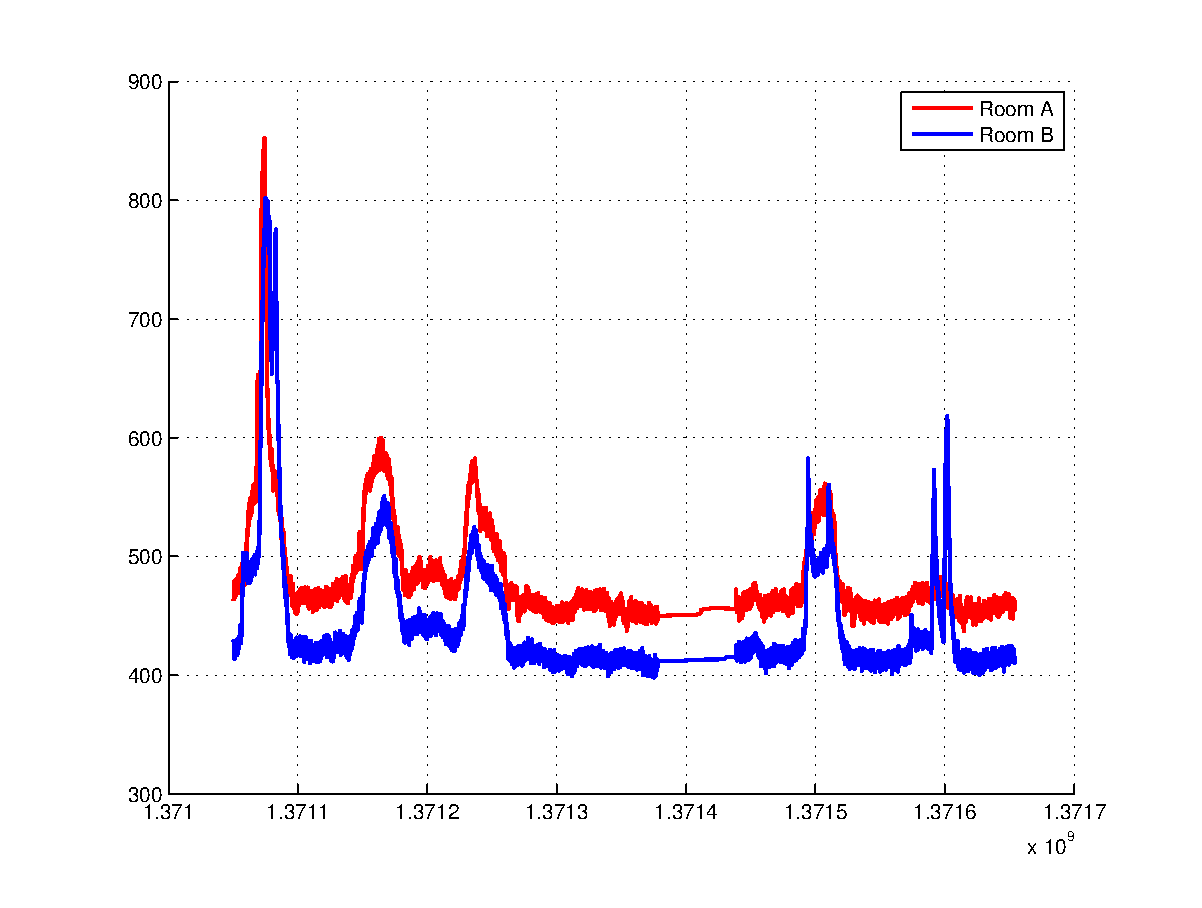
\includegraphics[width=0.48\textwidth]{figs/co2_pair.eps}
    \caption{CO2 sensor traces.}
\label{fig:co2traces}
\end{figure}

\begin{figure}[h!]
\centering
    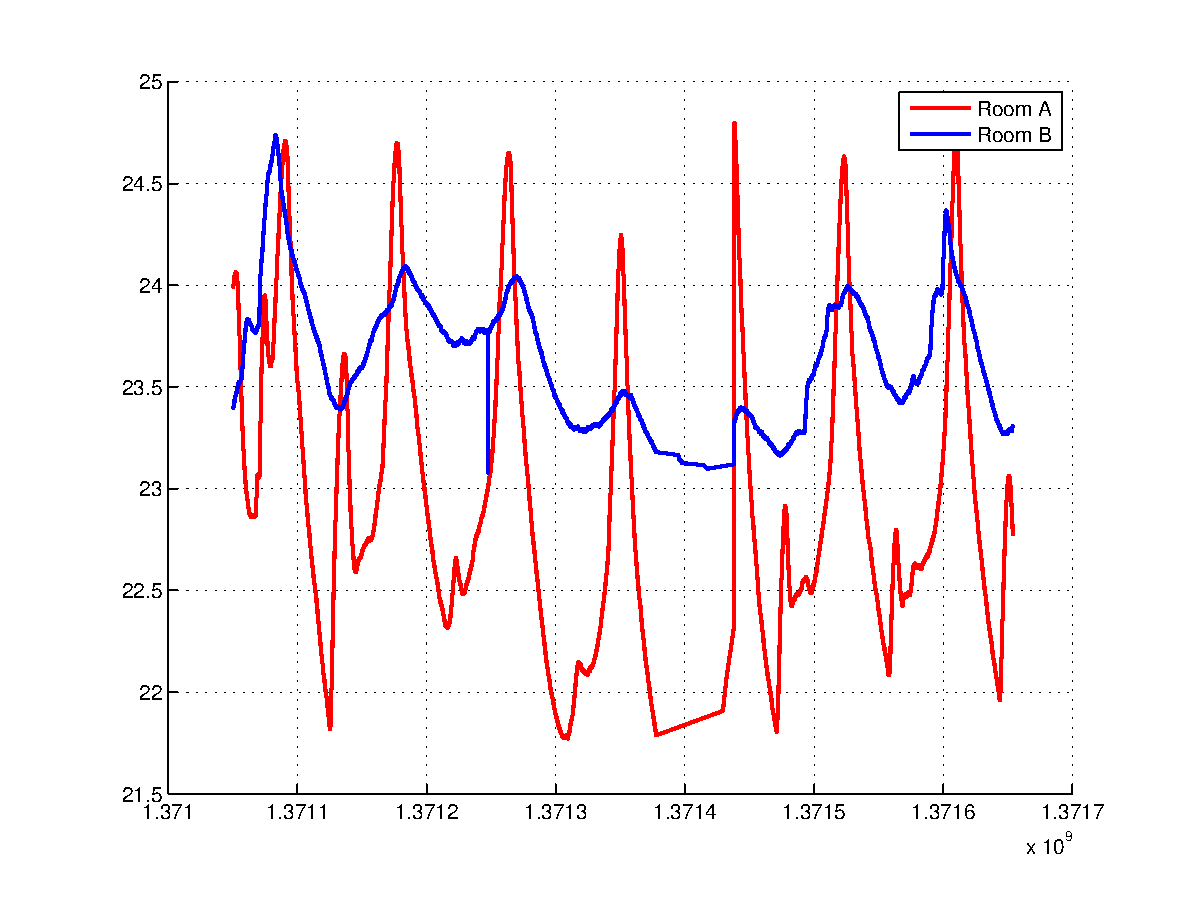
\includegraphics[width=0.48\textwidth]{figs/temp_pair.eps}
    \caption{temperature traces.}
\label{fig:temptraces}
\end{figure}


